\documentclass[10pt,a4paper]{ctexart}
\usepackage[margin=2cm]{geometry}
\usepackage{graphicx}
\usepackage{float}      % 支持 [H] 浮动体选项
\usepackage{hyperref}
\usepackage{multirow}
\usepackage{array}
\usepackage{caption}
\usepackage{amsmath}    % 提供方程环境
\usepackage{physics}    % 简化向量、微分算子语法
\newcommand{\myspace}[1]{\par\vspace{#1\baselineskip}} %自定义空一行
\usepackage{fancyhdr}
\usepackage{subcaption}
\pagestyle{fancy}
\fancyhf{}  % 清除所有页眉页脚
\fancyfoot[C]{\thepage}  % 在页脚中央设置页码
\renewcommand{\headrulewidth}{0pt}  % 去掉页眉横线
\renewcommand{\footrulewidth}{0pt}  % 去掉页脚横线

\usepackage{hyperref}
\hypersetup{
    colorlinks=true,
    linkcolor=blue,
    filecolor=magenta,      
    urlcolor=cyan,
    pdftitle={Overleaf Example},
    pdfpagemode=FullScreen,
    }

\usepackage{titlesec}

% 重新定义section格式
\titleformat{\section}
  {\normalfont\Large\bfseries}
  {\chinese{section}、}
  {0pt}
  {}

% 给出常用字号的自定义指令
\newcommand{\chuhao}{\fontsize{42pt}{48pt}\selectfont}
\newcommand{\xiaochu}{\fontsize{36pt}{42pt}\selectfont}
\newcommand{\xiaoer}{\fontsize{18pt}{21.6pt}\selectfont}
\newcommand{\sanhao}{\fontsize{16pt}{20pt}\selectfont}
\newcommand{\xiaosan}{\fontsize{15pt}{18pt}\selectfont}
\newcommand{\sihao}{\fontsize{14pt}{18pt}\selectfont}
\newcommand{\xiaosi}{\fontsize{12pt}{16pt}\selectfont}
\newcommand{\wuhao}{\fontsize{10.5pt}{12.6pt}\selectfont}

% 定义中文数字转换
\titleformat{\section}
  {\normalfont\Large\bfseries}
  {\zhnum{section}、}  % 使用\zhnum而不是\chinese
  {0pt}
  {}

% 标题设置
\title{\xiaochu\textbf{物理实验报告}}
\author{}
\date{}

\begin{document}

\vspace*{36pt} % 顶部空白

% 居中填写区域
\begin{center}
    
\includegraphics[width = 9cm]{figure/head.png}
    
    \xiaochu\textbf{物理实验报告}
    % 预留空白区域
    \vspace{13pt}
    \vspace{13pt}
    \vspace{13pt}
    \vspace{13pt}
    
    \sanhao\textbf{实验名称：\underline{\makebox[10cm]{ 交流电路功率因数实验、组装整流器}}} \\[10pt]
    \sanhao\textbf{实验桌号：\underline{\makebox[10cm]{ 6}}} \\[10pt]
    \sanhao\textbf{指导教师：\underline{\makebox[10cm]{ 王宗利 }}} \\[30pt]
    
    % 预留空白区域
    \myspace{6}
    
   \sihao\textbf{班级：\underline{\makebox[6cm]{}}} \\[10pt]
    \sihao\textbf{姓名：\underline{\makebox[6cm]{}}} \\[10pt]
    \sihao\textbf{学号：\underline{\makebox[6cm]{}}} \\[30pt]
    
   \sihao\textbf{实验日期: 
   \underline{\makebox[0.8cm]{2025}}  年 
   \underline{\makebox[0.4cm]{12}}月
   \underline{\makebox[0.4cm]{10}}日  
   星期\underline{\makebox[0.6cm]{三}}上午}
    
    \vspace{18pt}
    \sihao 浙江大学物理实验教学中心
    
\end{center}

\newpage

\section{预习报告}

    \subsection{实验综述}
    
    \xiaosi （自述实验现象、实验原理和实验方法，不超过300字，5分）
 
 1.交流电路功率因数实验
    交流电路中负载可以分为感性负载、容性负载和阻性负载。不同负载类型电压和电流相位差不同，阻性负载没有相位差，容性负载电流超前电压90°，
    感性负载电压超前电流90°。因此交流电功率$P=UI \cos(\phi)$，其中$\cos(\phi)$为功率因数。
     \begin{figure}[H]
        \centering
        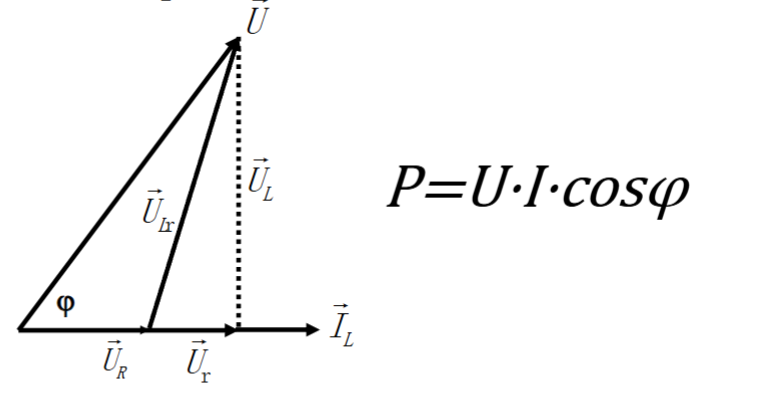
\includegraphics[width=0.6\textwidth]{figure/preview_2.png}
        \caption{功率因数示意图}
        \label{fig:power_factor}
    \end{figure}
    通过在感性负载两端并联电容可以减小$\phi$，提高功率因数。
    \begin{figure}[H]
        \centering
        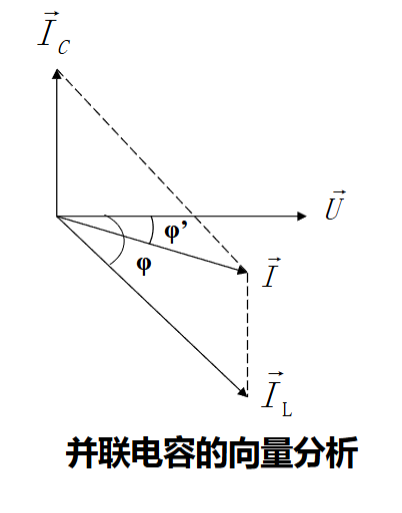
\includegraphics[width=0.6\textwidth]{figure/preview_1.png}
        \caption{并联电容可以提高功率因数示意图}
        \label{fig:power_factor_capacitor}
    \end{figure}
    实验通过改变并联电容大小，测量电流、电压和功率，计算功率因数，拟合功率因数和电容的关系，寻找最佳电容值使功率因数最大。

    实验中使用日光灯作为感性负载。

    2.组装整流器

二极管具有单向导电性，以此为基本原理可以构建整流电路。不同的连接方式可以实现半波整流和全波整流。

    实验中通过组装二极管、电阻、电容等元件，组装成半波和全波整流电路，测量输出电压波形以及平均值、有效值，分析整流效果。

    电容和电感有充放电特性，可以构建滤波电路。实验中通过不使用滤波器和使用不同电容值的滤波器，测量输出波形，分析滤波效果。
    实际生活中整流电路和滤波电路更复杂。也不止包含整流电路和滤波电路，还包含稳压电路等，以满足不同电子设备对电源的要求。
    \begin{figure}[H]
        \centering
        
\includegraphics[width=0.6\textwidth]{figure/circuit.png}
        \caption{电路示意图}
        \label{fig:rectifier_filter}    
    \end{figure}
\myspace{2}
    \subsection{实验重点}
    
    \xiaosi（简述本实验的学习重点，不超过100字，3分）
    
(1)理解交流电功率因数的概念及其对电路性能的影响。

(2)掌握通过并联电容提高功率因数的方法及其原理。

(3)理解二极管的单向导电特性及其在整流电路中的应用。

(4)掌握组装半波和全波整流电路的方法及滤波电路的基本原理。
    \myspace{2}
    
    \subsection{实验难点}
    
    \xiaosi（简述本实验的实现难点，不超过100字，2分）

(1)准确测量交流电路中的电压、电流和功率，计算功率因数。

(2)正确选择并联电容值以优化功率因数。

(3)熟练组装整流电路，确保电路连接正确无误。

(4)分析整流和滤波效果，理解不同滤波器参数对输出波形的影响。
\myspace{2}
\section{原始数据}

    \xiaosi （将有老师签名的“自备数据记录草稿纸”的扫描或手机拍摄图粘贴在下方，20分）
   \begin{figure}[H]
    \centering
    
\includegraphics[width=0.8\textwidth]{figure/raw_data.jpg}
    \caption{实验数据原始记录}  
\end{figure}

\section{结果与分析}

    \subsection{数据处理与结果}
    \xiaosi （列出数据表格、选择数据处理方法、给定测量或计算结果，30分）

    1.交流电路功率因数实验
    
   打开总电源开关，开启日光灯开关，观察日光灯启动过程。用电压表、电流表、功率表测量日光灯电路在额定电压时电路的功率、各电压、电流，并计算功率因数。记录实验数据。接入电容，并按照电容值从小容量到大容量变化，测量各电流、电压、功率随电容变化的规律，将测量数据记入表中如下所示。
\begin{table}[H]
\centering
\caption{交流电功率因数数据记录表格}
\begin{tabular}{|c|c|c|c|c|c|c|c|c|c|}
\hline
   & $1 \mu F$ & $2 \mu F$ & $3 \mu F$ & $4 \mu F$ & $5 \mu F$ & $6 \mu F$ & $7 \mu F$ & $8 \mu F$ & $9 \mu F$ \\ \hline
I(A) & 0.2435 & 0.1879 & 0.1434 & 0.1319 & 0.1369 & 0.1602 & 0.2091 & 0.2547 & 0.3192 \\ \hline
U(V) & 219.5 & 219.5 & 219.7 & 219.2 & 219.1 & 218.9 & 219.5 & 219.5 & 219.5 \\ \hline
P(W) & 25.6 & 25.7 & 25.8 & 25.6 & 25.8 & 25.9 & 26.1 & 26.4 & 26.5 \\ \hline
$\cos \phi$ & 0.48 & 0.62 & 0.82 & 0.89 & 0.86 & 0.74 & 0.57 & 0.47 & 0.38 \\ \hline
\end{tabular}
\end{table}
拟合功率因数和电容的关系曲线如下图所示：
\begin{figure}[H]
    \centering
    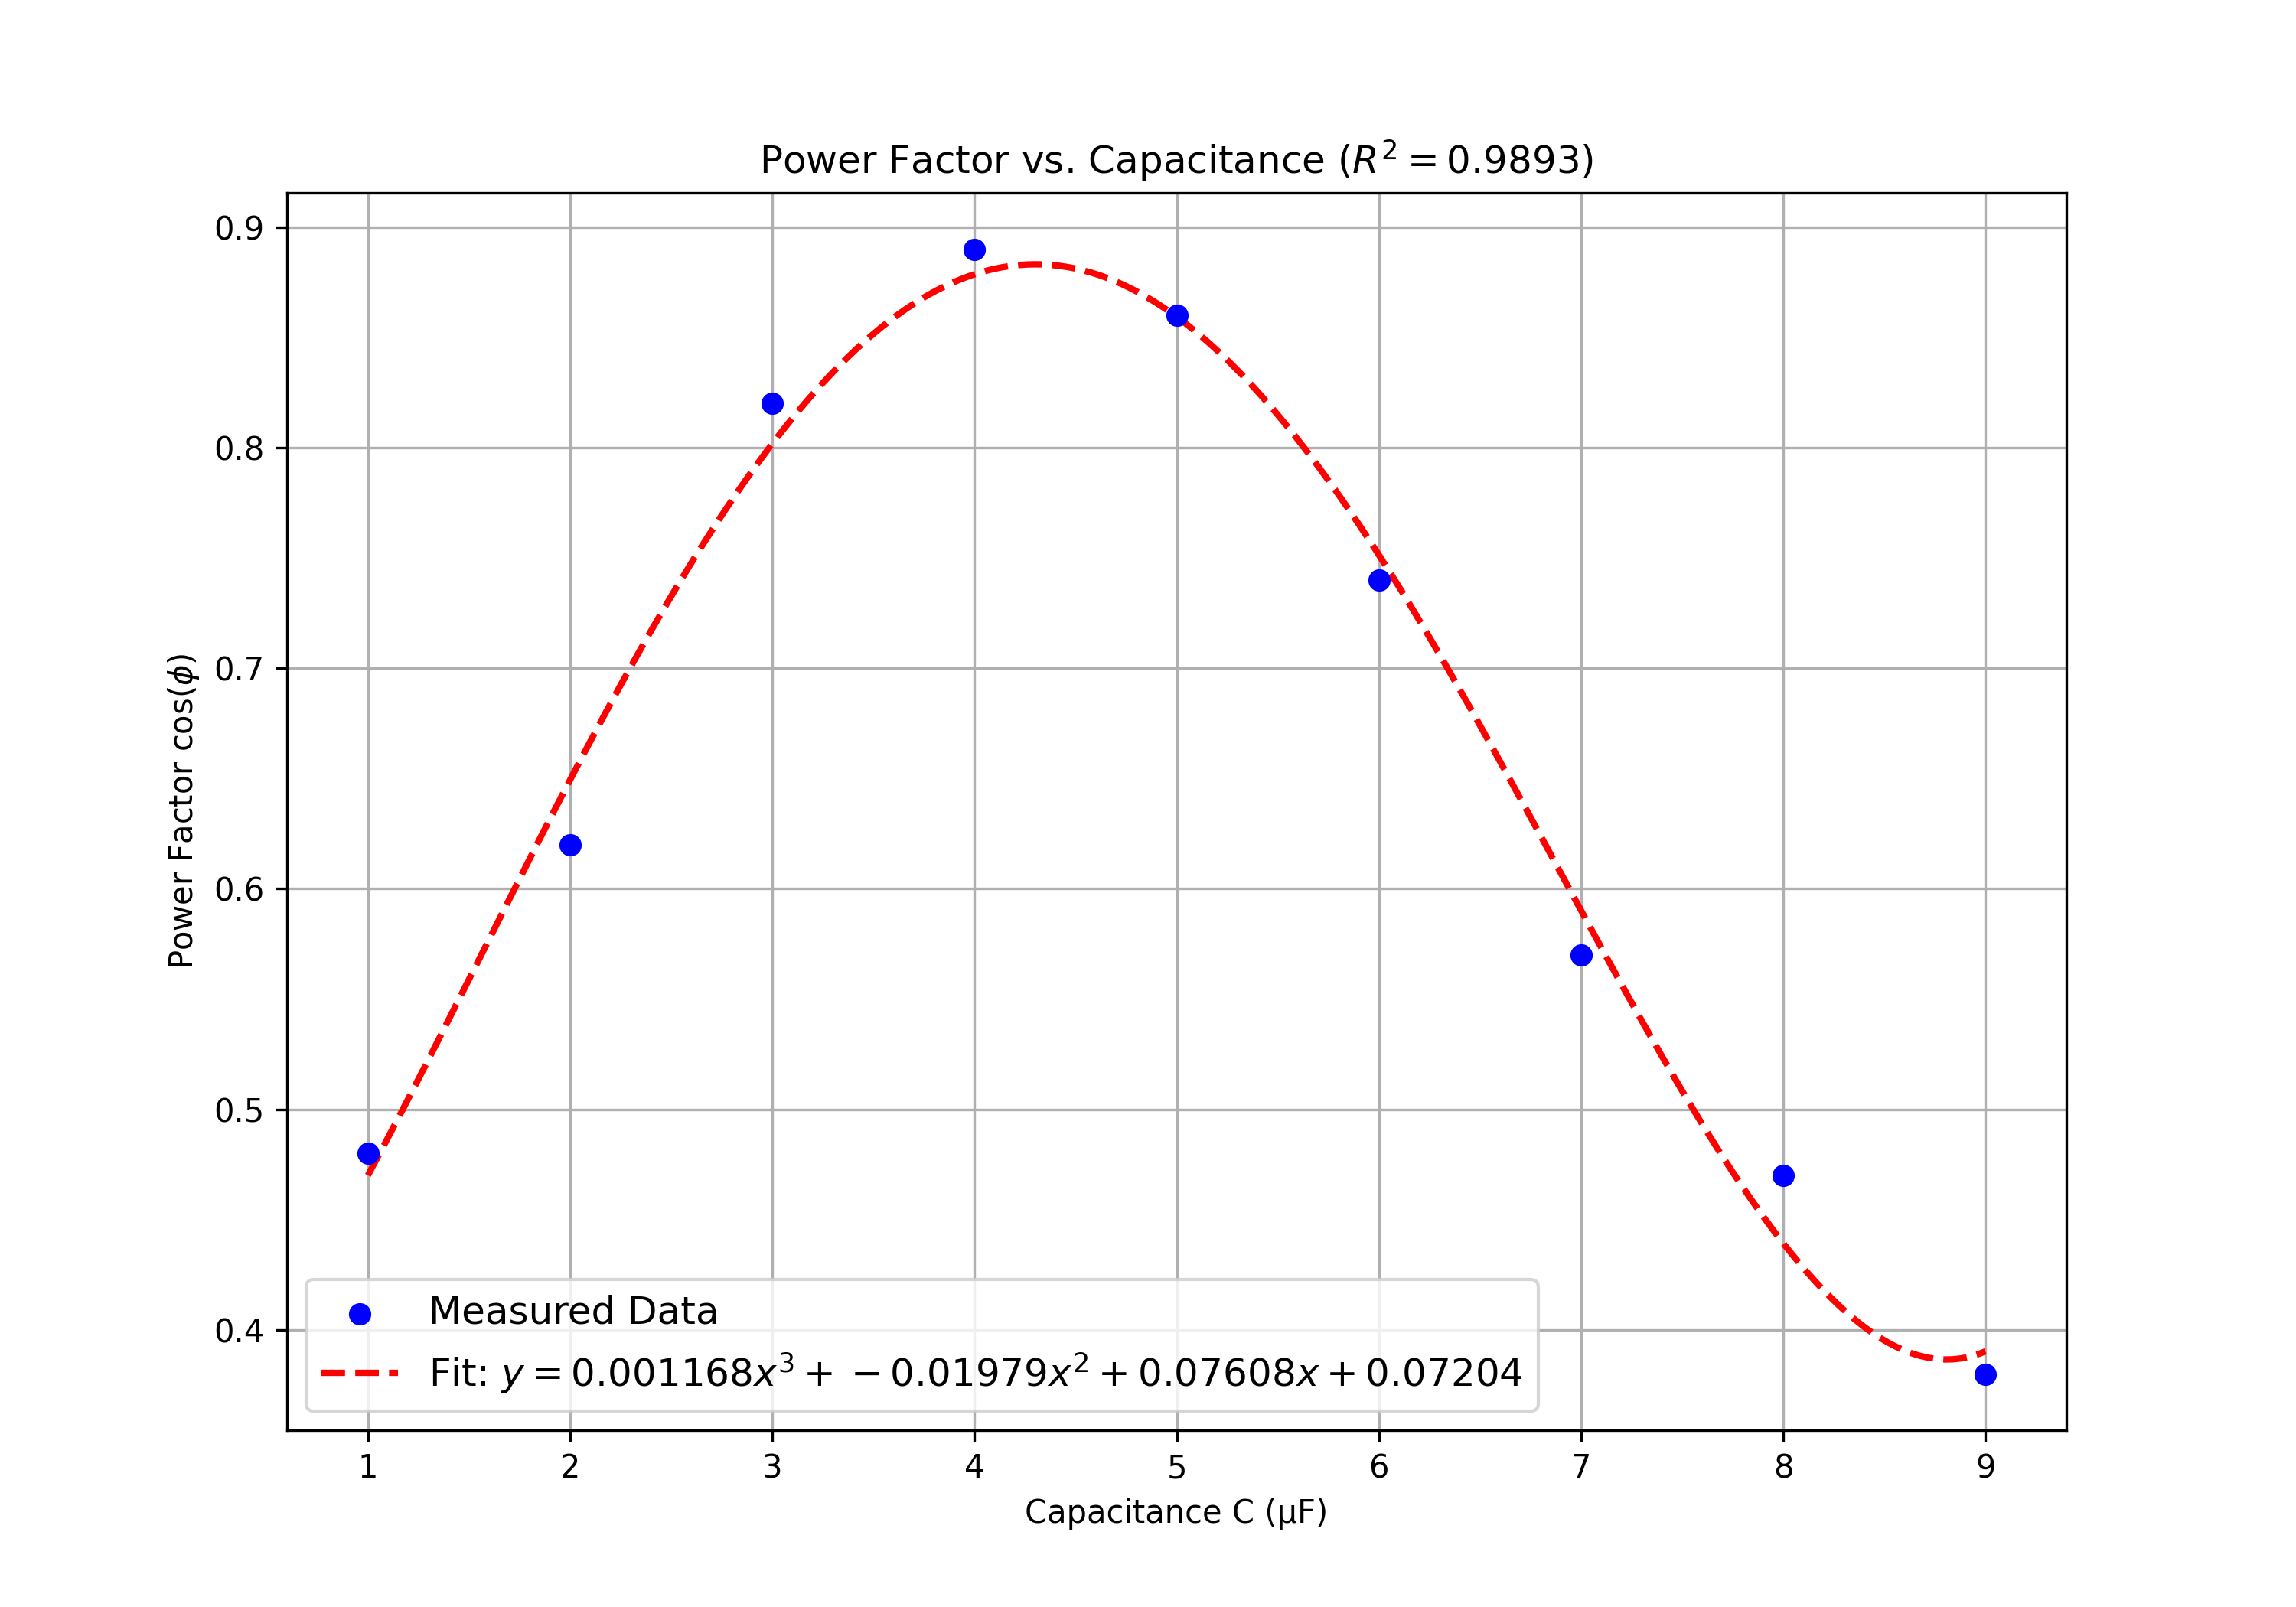
\includegraphics[width=0.6\textwidth]{figure/power_factor_fit.png}
    \caption{功率因数与电容关系曲线拟合}
    \label{fig:power_factor_fit}
\end{figure}
由图可见，功率因数随电容增大先增大后减小，使功率因数为最大值时的电容值可以近似认为是$4 \mu F$，此时功率因数为0.89，功率为25.6W。


2.组装整流器

组装不同整流电路，并分别测量输入信号波形、有效值、峰峰值，输出信号波形、平均值等相关信息。

之后在电路中加入滤波器来观察滤波器前后波形变化。

最终计算转换系数$k=\frac{\overline{u_0}}{u_2}$，并与理论值进行对比，计算相对误差,填入下表。
\begin{table}[H]
\centering
\caption{整流电路类型及输出信号分析}
\begin{tabular}{|c|c|c|c|}
\hline
& 单相半波 & 单相全波 & 桥式 \\ \hline
输入电压有效值$u_2$ (V) & 13.35 & 12.21 & 11.74 \\ \hline
输入电压峰峰值$u_{2(pp)}$ (V) & 38.40 & 35.20 & 34.00 \\ \hline
输入电压波形 &见图\ref{fig:i1} & 见图\ref{fig:i2} & 见图\ref{fig:i3} \\ \hline
输出电压平均值$\overline{u_0}$ (V) & 5.530 & 9.890 & 9.234 \\ \hline
输出电压波形（滤波前） & 见图\ref{fig:o1} & 见图\ref{fig:o2} & 见图\ref{fig:o3} \\ \hline
输出电压波形（滤波后） & 见图\ref{fig:f1} & 见图\ref{fig:f2} & 见图\ref{fig:f3} \\ \hline
转换系数测量值 $k$ & 0.41 & 0.39 & 0.79 \\ \hline
理论值 $k$ & 0.45 & 0.90 & 0.90 \\ \hline
转化系数相对误差   &   8\%  &  10\%    &  12\% \\ \hline
\end{tabular}
\end{table}
输入信号波形草图如下：
\begin{figure}[H]
    \centering
    \begin{subfigure}[u]{0.32\textwidth}
        \centering
        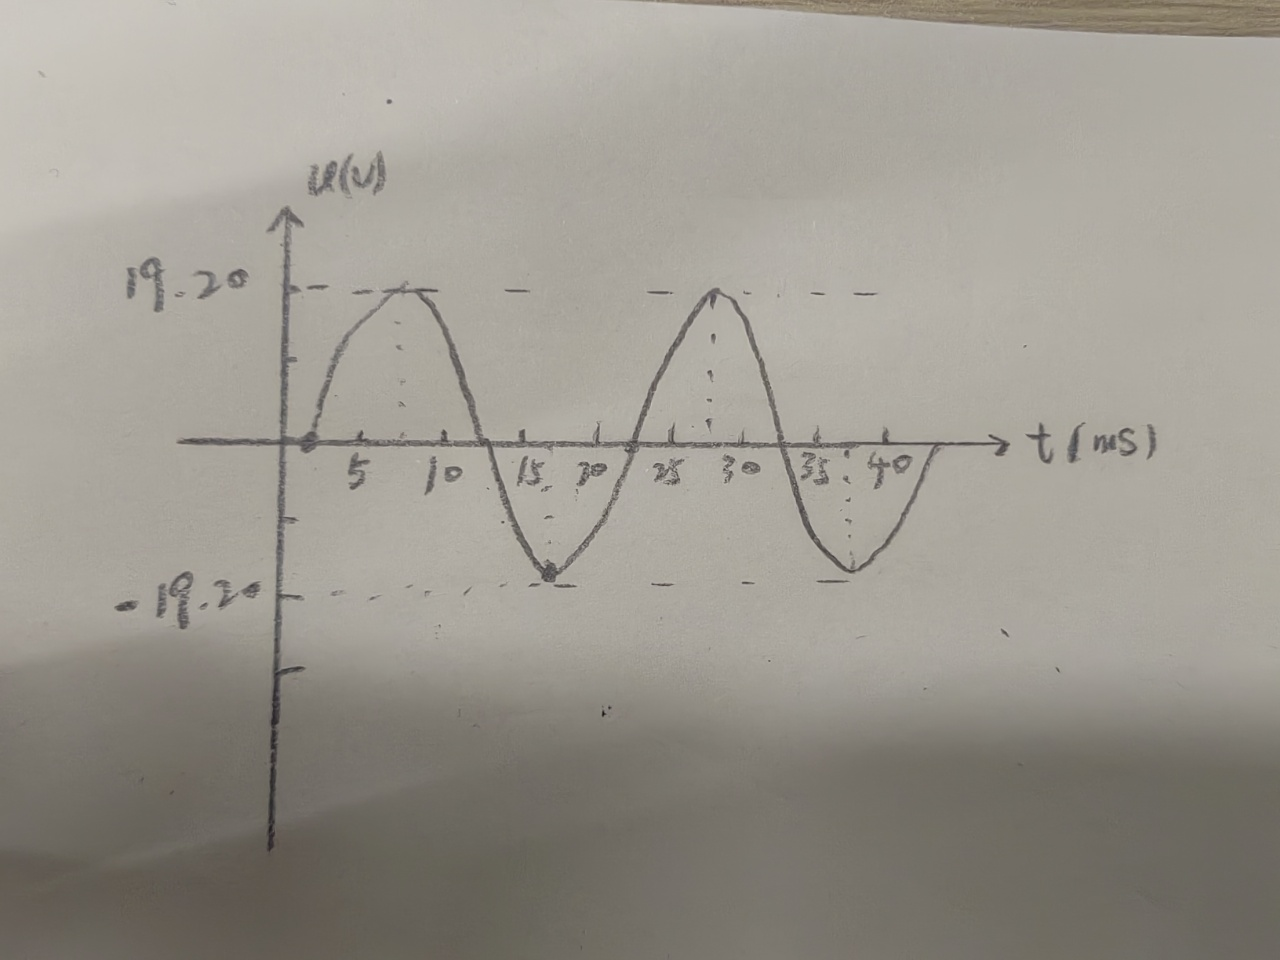
\includegraphics[width=\textwidth]{figure/waveform_1_input.jpg}
        \caption{单相半波整流电路输入信号波形草图}
        \label{fig:i1}
    \end{subfigure}
    \hfill
    \begin{subfigure}[u]{0.32\textwidth}
        \centering
        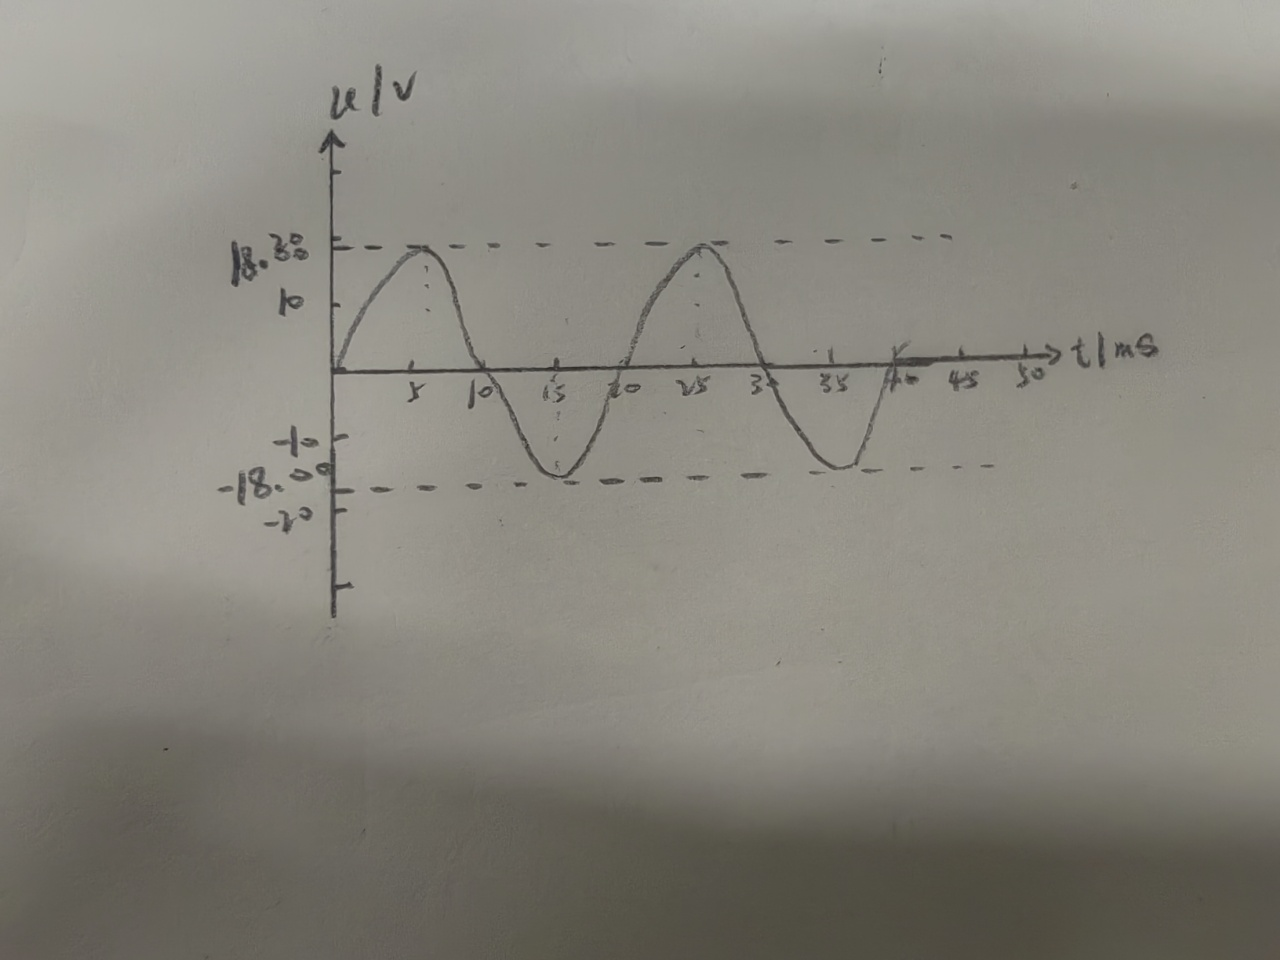
\includegraphics[width=\textwidth]{figure/waveform_2_input.jpg}
        \caption{单相全波整流电路输入信号波形草图}
        \label{fig:i2}
    \end{subfigure}
    \hfill
    \begin{subfigure}[u]{0.32\textwidth}
        \centering
        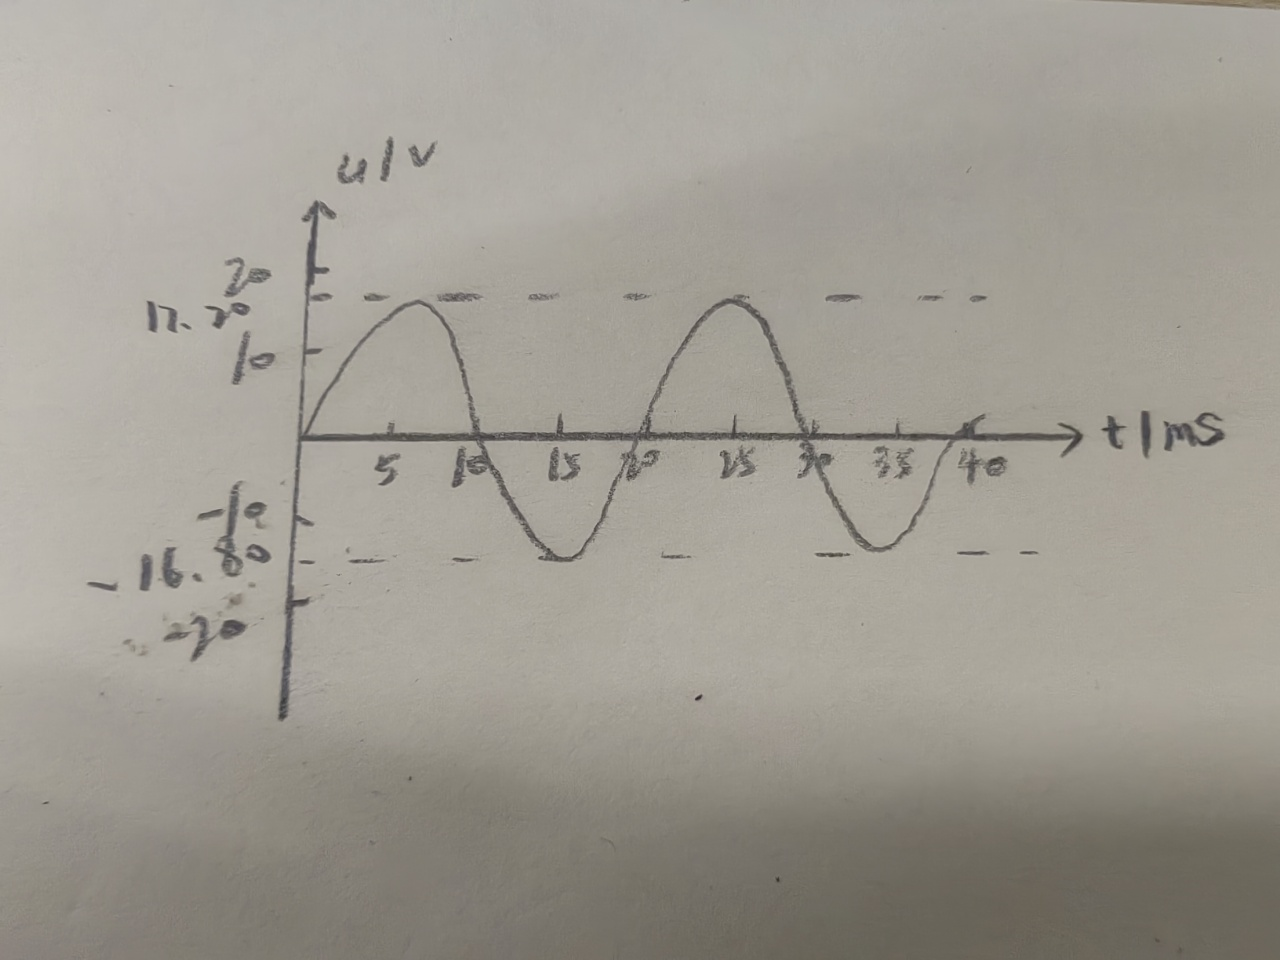
\includegraphics[width=\textwidth]{figure/waveform_3_input.jpg}
        \caption{桥式整流电路输入信号波形图}
        \label{fig:i3}
    \end{subfigure}
    \caption{输入信号波形草图}
    \label{fig:i}
\end{figure}
输出信号波形草图如下：
\begin{figure}[H]
    \centering
    \begin{subfigure}[b]{0.32\textwidth}
        \centering
        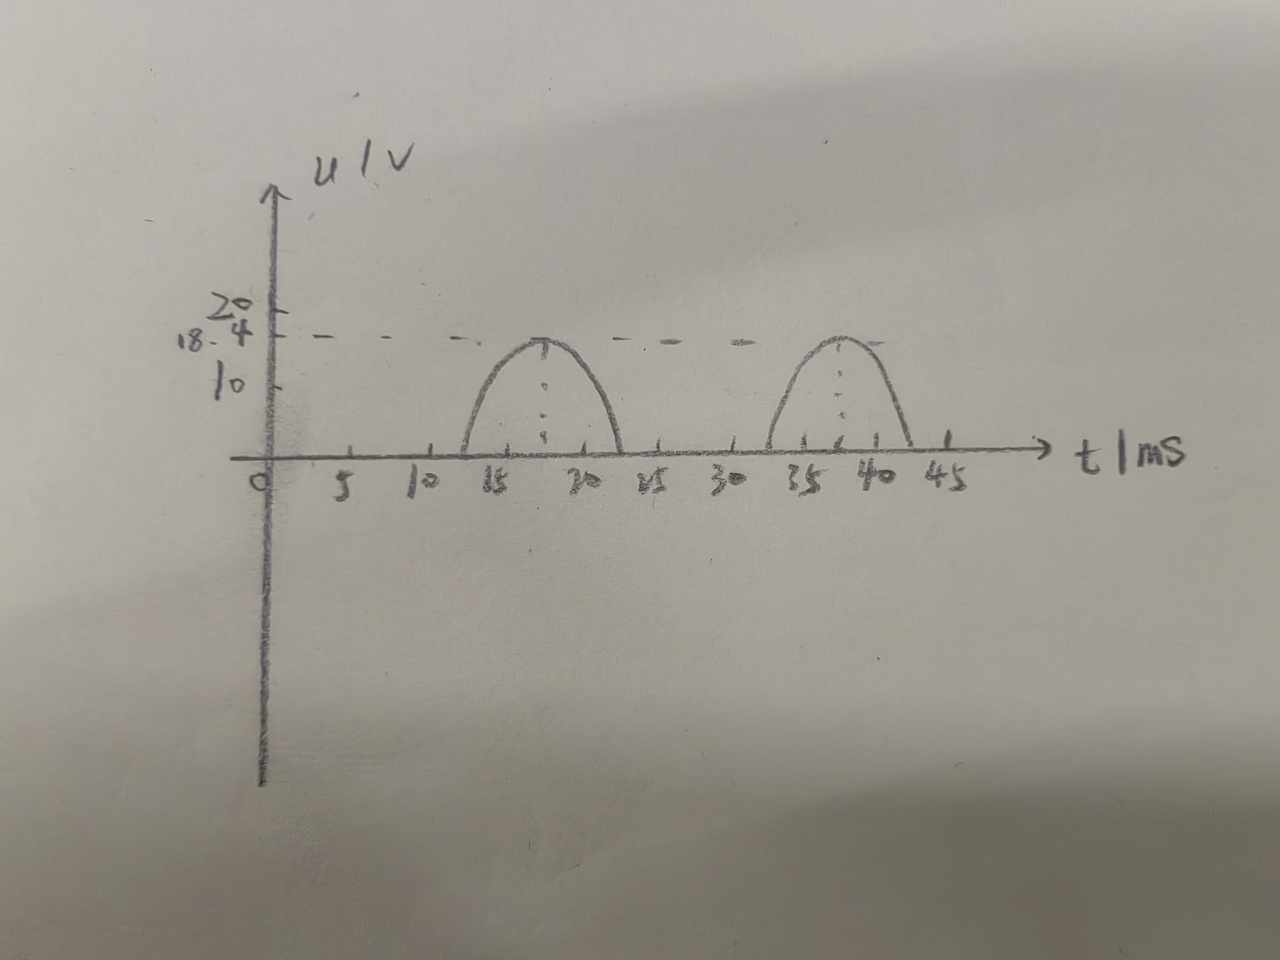
\includegraphics[width=\textwidth]{figure/waveform_1_output.jpg}
        \caption{单相半波整流电路输出信号波形草图}
        \label{fig:o1}
    \end{subfigure}
    \hfill
    \begin{subfigure}[b]{0.32\textwidth}
        \centering
        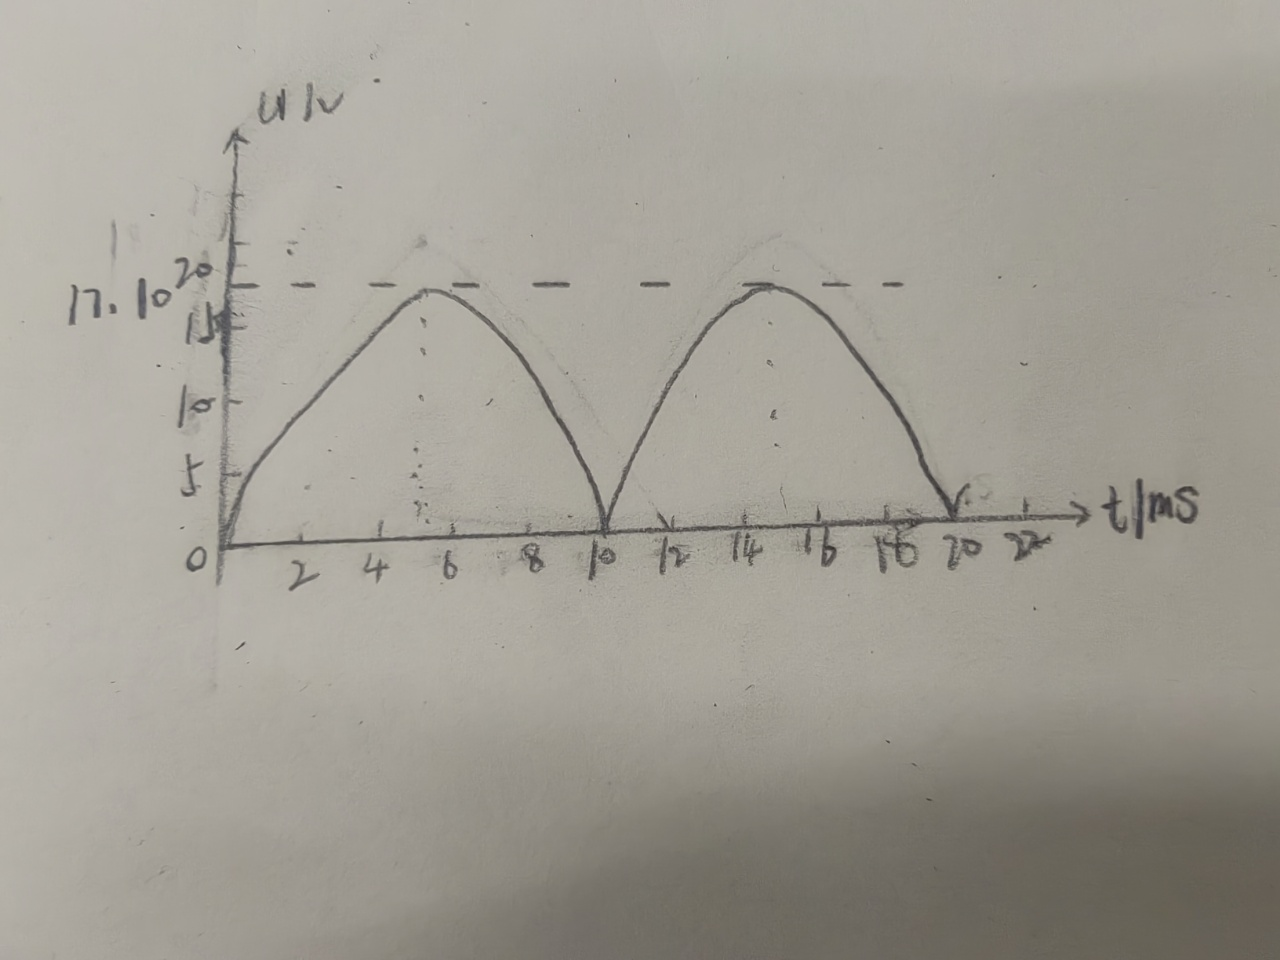
\includegraphics[width=\textwidth]{figure/waveform_2_output.jpg}
        \caption{单相全波整流电路输出信号波形草图}
        \label{fig:o2}
    \end{subfigure}
    \hfill
    \begin{subfigure}[b]{0.32\textwidth}
        \centering
        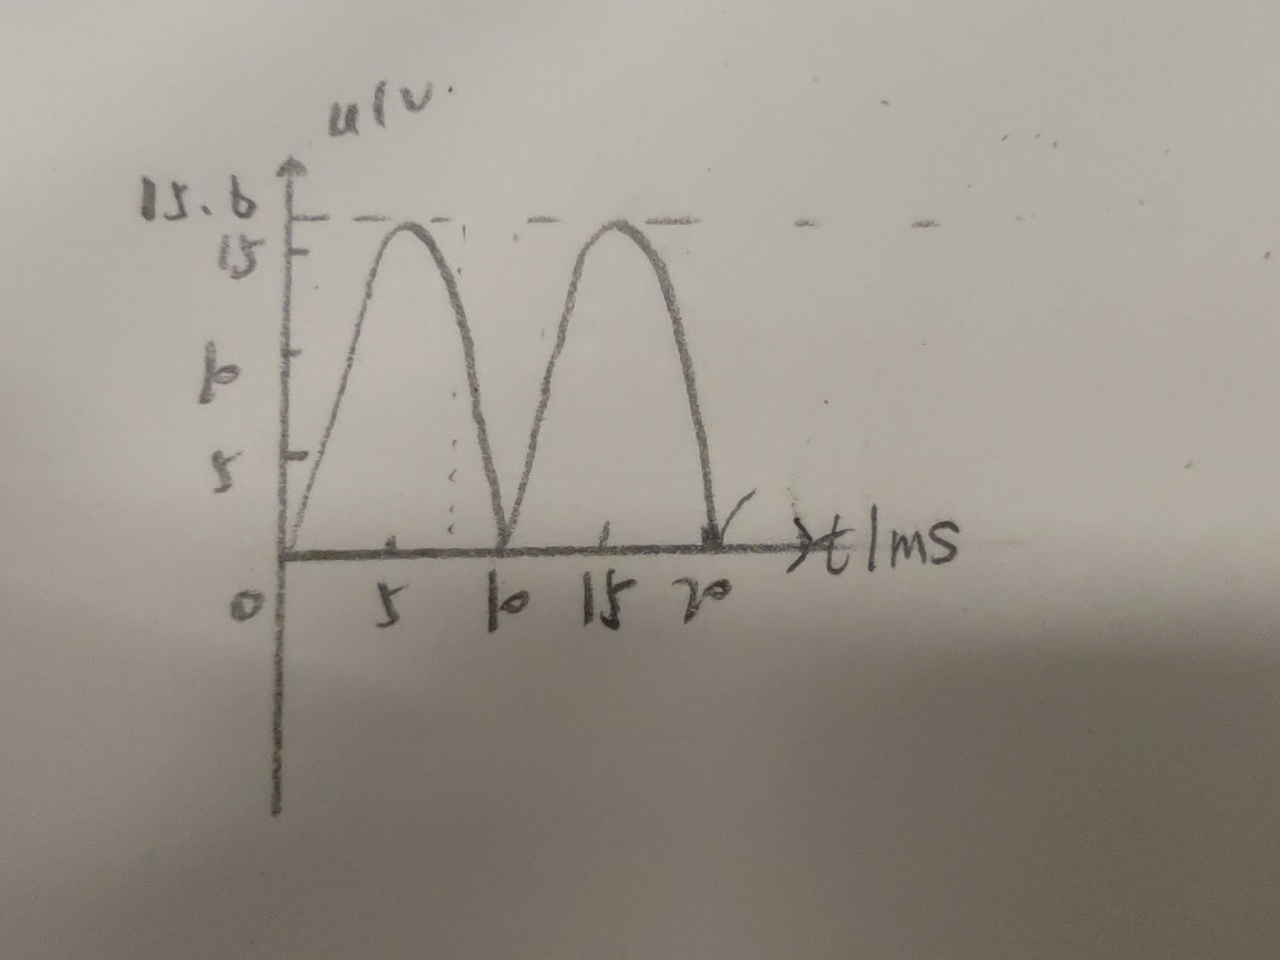
\includegraphics[width=\textwidth]{figure/waveform_3_output.jpg}
        \caption{桥式整流电路输出信号波形图}
        \label{fig:o3}
    \end{subfigure}
    \caption{输出信号波形草图}
    \label{fig:o}
\end{figure}

输出信号滤波的波形草图如下：
\begin{figure}[H]
    \centering
    \begin{subfigure}[b]{0.32\textwidth}
        \centering
        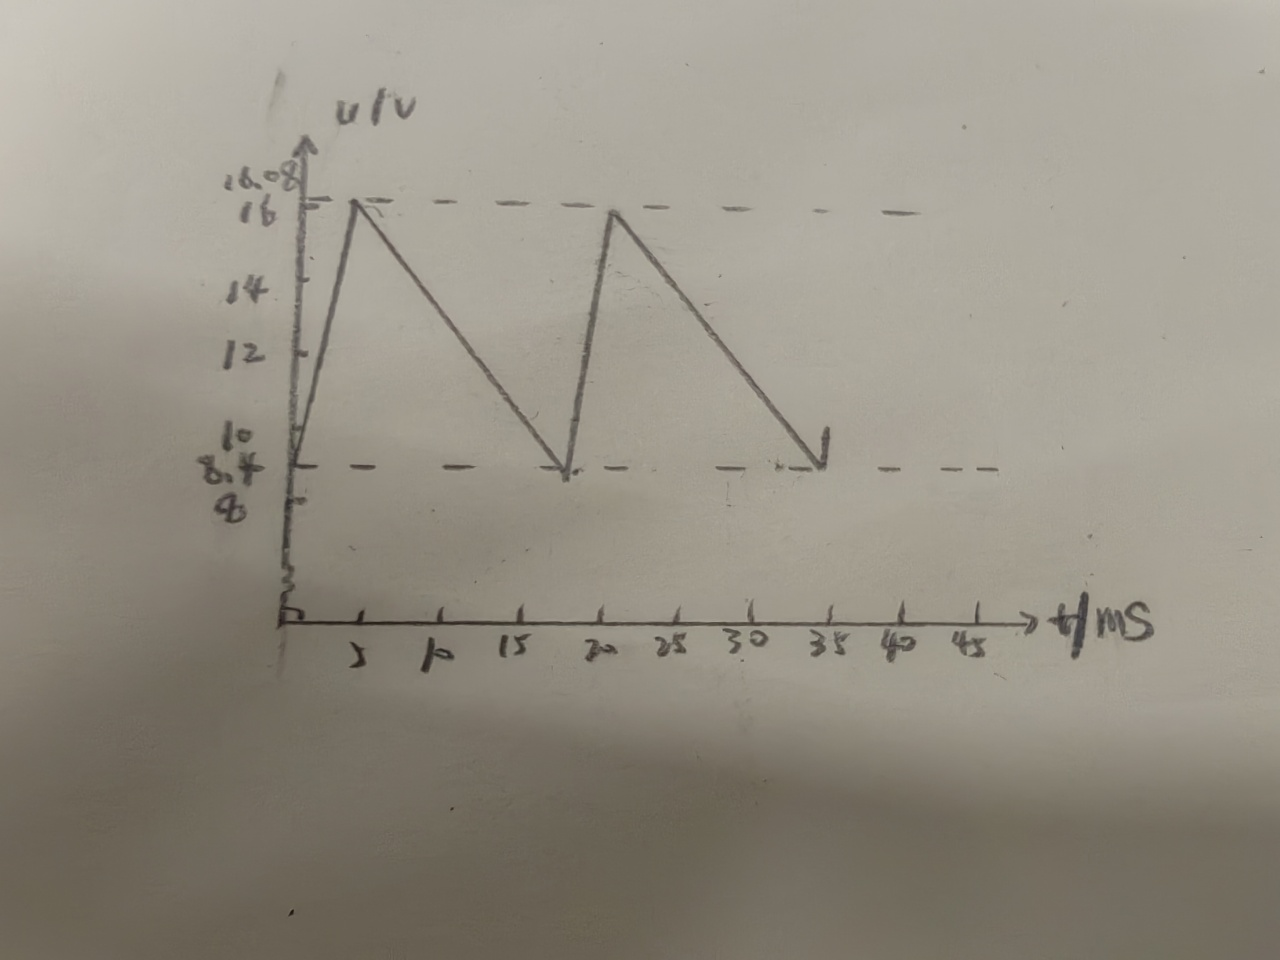
\includegraphics[width=\textwidth]{figure/waveform_1_f.jpg}
        \caption{单相半波整流电路输出信号滤波波形草图}
        \label{fig:f1}
    \end{subfigure}
    \hfill
    \begin{subfigure}[b]{0.32\textwidth}
        \centering
        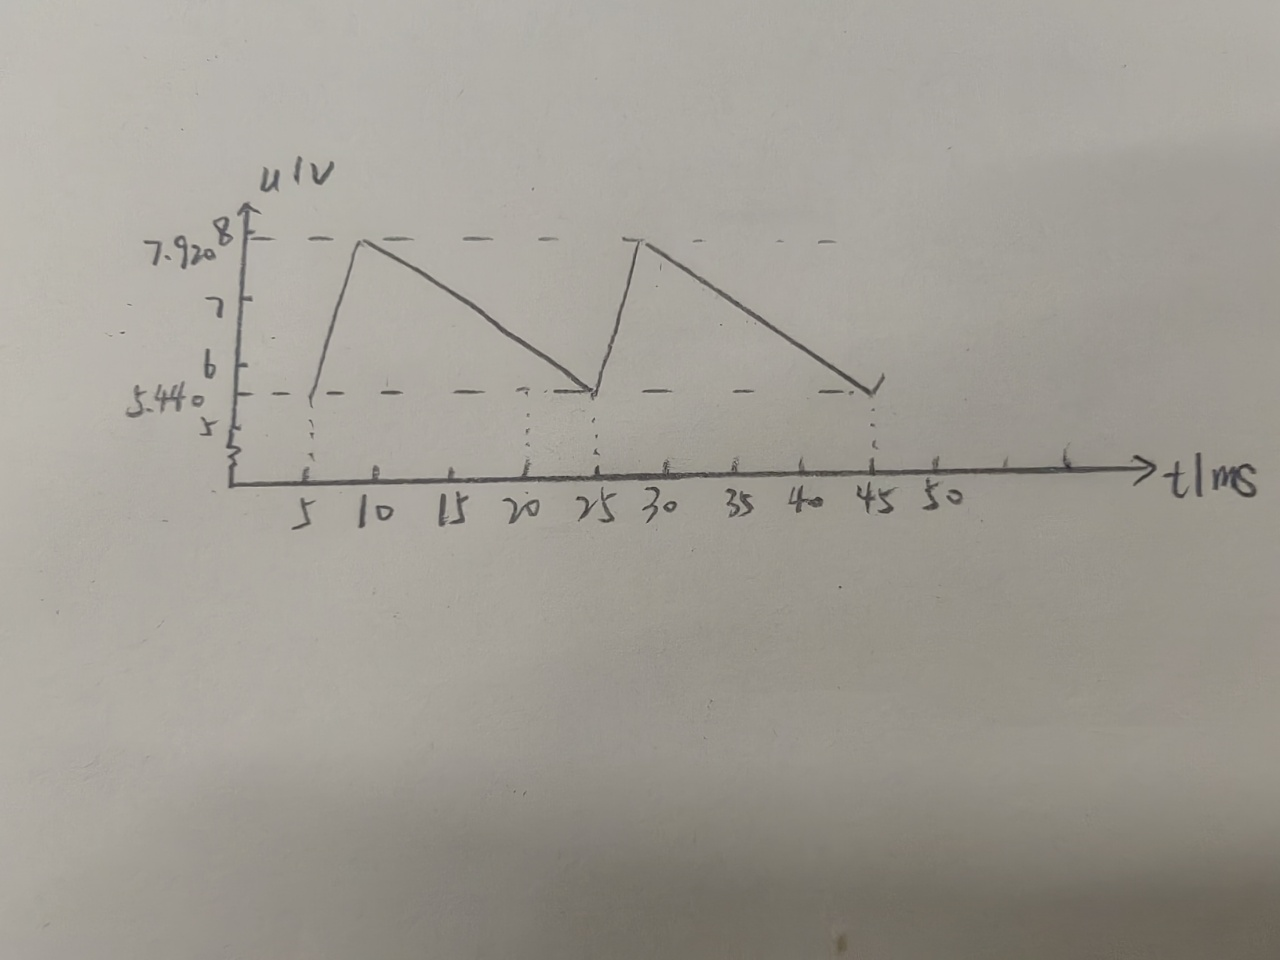
\includegraphics[width=\textwidth]{figure/waveform_2_f.jpg}
        \caption{单相全波整流电路输出信号滤波波形草图}
        \label{fig:f2}
    \end{subfigure}
    \hfill
    \begin{subfigure}[b]{0.32\textwidth}
        \centering
        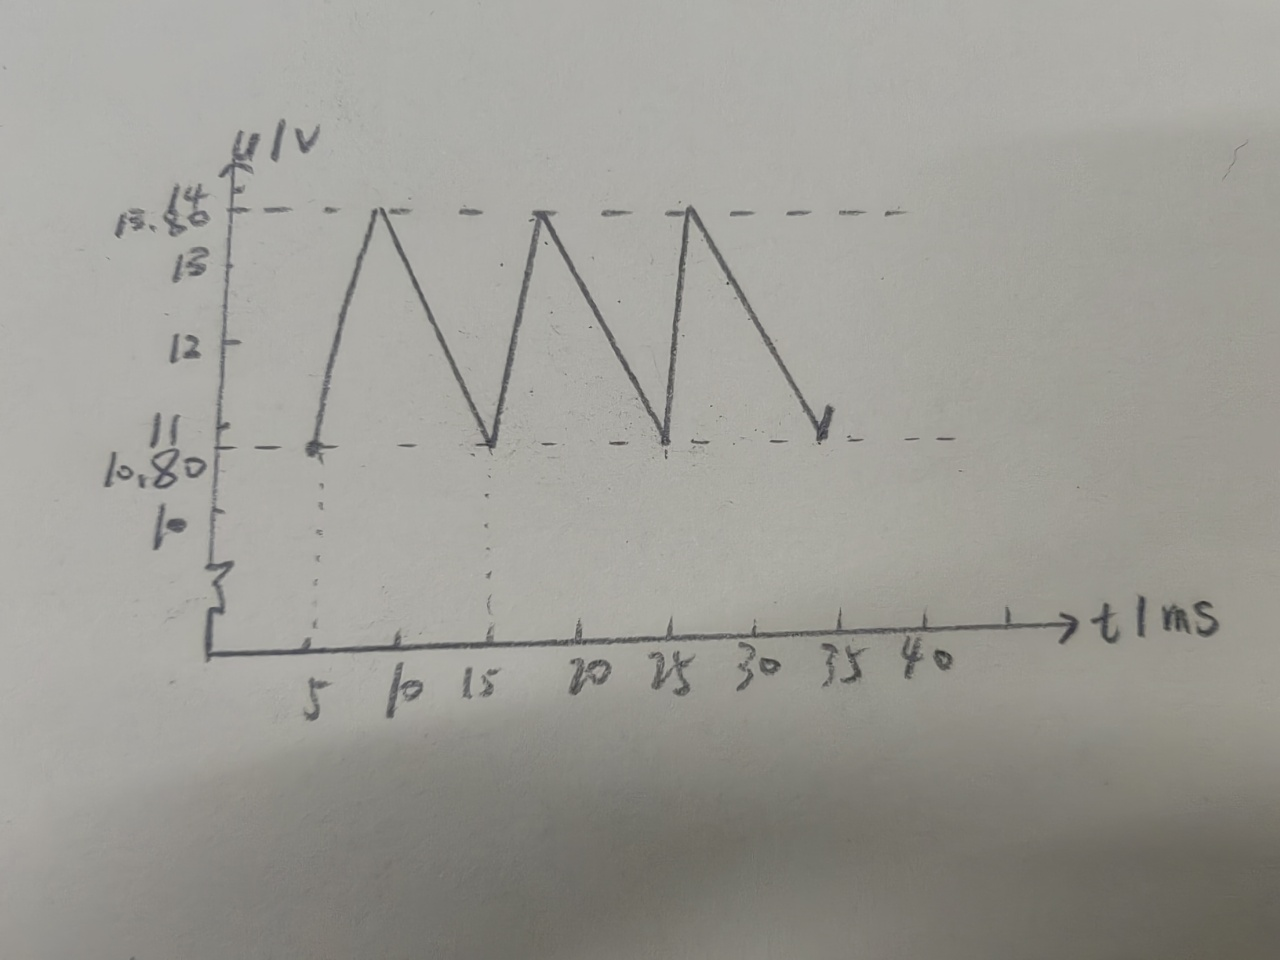
\includegraphics[width=\textwidth]{figure/waveform_3_f.jpg}
        \caption{桥式整流电路输出信号滤波波形图}
        \label{fig:f3}
    \end{subfigure}
    \caption{输出信号滤波波形草图}
    \label{fig:f}
\end{figure}

    \myspace{2}
\subsection{误差分析}
    \xiaosi （运用测量误差、相对误差、不确定度等分析实验结果，20分）

    \begin{enumerate}
        \item \textbf{仪器误差}：电压表、电流表和功率表的精度限制导致的测量误差。
        \item \textbf{读数误差}:模拟仪表读取时的人为估读误差，约为最小分度的1/5。
        \item \textbf{环境因素}：实验室温度、湿度变化可能影响元件参数（特别是电容的容值）和仪器工作状态。
        \item \textbf{标称值不准确}:实际电容值、电阻值与标称值存在偏差，影响计算结果。
        \item \textbf{理论计算误差}:理论模型简化，未考虑元件的非理想特性，如二极管的正向压降、寄生电感电容等。二极管正向压降（约0.7V）的影响，理论计算转换系数时未考虑
    \end{enumerate}
    \myspace{1}
    \subsection{实验探讨}
    \xiaosi （对实验内容、现象和过程的小结，不超过100字，10分）
    
    本实验验证了并联电容提高功率因数的原理，确定了日光灯电路的最佳补偿电容为$4\mu F$。通过组装整流电路，观察到不同电路结构的整流效果差异，验证了滤波电路对输出波形平滑度的改善作用。实验结果表明，理论分析与实际测量基本相符，误差在合理范围内。

\section{思考题}

    \xiaosi （解答教材或讲义或老师布置的思考题，10分）
    
    \textbf{1. 提高功率因数的意义何在？为什么并联电容能提高功率因数？并联的电容是否越大越好？}
    
    提高功率因数的意义在于：
    \begin{enumerate}
        \item \textbf{提高电源利用率}：在相同视在功率下，提高功率因数可以输送更多有功功率
        \item \textbf{减少线路损耗}：降低无功电流，减少传输过程中的能量损失
        \item \textbf{改善电压质量}：减少线路压降，提高供电质量
    \end{enumerate}
    
    并联电容能提高功率因数的原因：感性负载电流滞后电压，而电容电流超前电压90°，二者相位相反。并联电容后，电容电流抵消部分电感电流，使总电流与电压相位差减小，从而提高功率因数。
    
    并联电容并非越大越好。当电容过小时补偿不足；当电容过大时，电路变为容性，功率因数反而下降，出现过补偿现象。最佳补偿电容应使电路接近阻性，功率因数接近1。
    
    \textbf{2. 在实验中，随着电容增加，电路总电流的变化规律为由大变小再变大，试分析原因。}
    
    未加电容时电路呈感性，总电流较大。随着电容增加，电容电流$I_C$与电感电流$I_L$相位相反，总电流$I=\sqrt{I_R^2+(I_L-I_C)^2}$逐渐减小。当$I_C=I_L$时发生完全补偿，总电流最小（等于电阻电流）。继续增大电容，$I_C>I_L$，电路呈容性，总电流再次增大。
    
    \textbf{3. 在进行功率因数补偿时，本实验采用并联电容器的方法，为什么不采用串联电容器的方法？}
    
    原因如下：
    \begin{enumerate}
        \item \textbf{改变电路特性}：串联电容会改变负载阻抗，可能影响设备正常工作
        \item \textbf{电压分配问题}：串联电容会分压，降低负载端电压
        \item \textbf{安全性}：串联电容故障（如击穿）会导致电路中断，影响设备运行
        \item \textbf{补偿效果}：并联电容仅补偿无功功率，不改变有功功率；串联电容会影响有功功率传输
    \end{enumerate}
    
    \textbf{4. 总结不同整流电路和不同滤波电路的利弊。}
    
    \begin{table}[H]
    \centering
    \caption{不同整流电路对比}
    \begin{tabular}{|c|c|c|c|}
    \hline
    类型 & 优点 & 缺点 & 适用场合 \\ \hline
    半波整流 & 电路简单，元件少 & 效率低，纹波大 & 小功率、低成本应用 \\ \hline
    全波整流 & 效率较高，纹波较小 & 需要中心抽头变压器 & 中等功率应用 \\ \hline
    桥式整流 & 效率高，无需中心抽头 & 需要4个二极管，压降大 & 广泛适用 \\ \hline
    \end{tabular}
    \end{table}
    
    \begin{table}[H]
    \centering
    \caption{不同滤波电路对比}
    \begin{tabular}{|c|c|c|c|}
    \hline
    类型 & 优点 & 缺点 & 适用场合 \\ \hline
    电容滤波 & 电路简单，体积小 & 输出电流能力差 & 小电流、高电压场合 \\ \hline
    电感滤波 & 带载能力强，适用于大电流 & 体积大，成本高 & 大电流场合 \\ \hline
    LC滤波 & 滤波效果好，纹波小 & 体积大，设计复杂 & 要求较高的场合 \\ \hline
    \end{tabular}
    \end{table}
    
    \textbf{5. 整流和滤波的目的分别是什么？}
    
    \textbf{整流目的}：将交流电转换为单向脉动的直流电，利用二极管的单向导电性实现电流方向的控制。
    
    \textbf{滤波目的}：减小整流后输出电压的脉动（纹波），获得平滑的直流电压，使输出电压更稳定。
    
    \textbf{6. 如何根据需要选择合适的整流电路？}
    
    选择整流电路应考虑以下因素：
    \begin{enumerate}
        \item \textbf{功率需求}：小功率可选半波整流，中、大功率应选全波或桥式整流
        \item \textbf{成本限制}：半波整流成本最低，桥式整流元件较多但性能好
        \item \textbf{变压器条件}：如有中心抽头变压器可选全波整流，否则选桥式整流
        \item \textbf{效率要求}：桥式整流效率最高，半波整流效率最低
        \item \textbf{纹波要求}：要求纹波小的场合应选择全波或桥式整流
        \item \textbf{空间限制}：考虑元件的体积和散热要求
    \end{enumerate}
    综合而言，桥式整流因其性能优良、适应性强而成为最常用的整流方案。

\newpage

\sihao\textbf{注意事项：}
\xiaosi
\begin{enumerate}
    \item 用PDF格式上传“实验报告”，文件名：学生姓名+学号+实验名称+周次。
    \item  “实验报告”必须递交在“学在浙大”的本课程的对应实验项目的“作业”模块内。
    \item  “实验报告”成绩必须在“浙江大学物理实验教学中心网站”-“选课系统”内查询。
    \item 教学评价必须在“浙江大学物理实验教学中心网站”-“选课系统”内进行，学生必须进行教学评价，才能看到实验报告成绩，教学评价必须在本次实验结束后 3 天内进行。
\end{enumerate}

\vspace{1cm}
\xiaosi\centering \textbf{浙江大学物理实验教学中心制}

\end{document}